\newglossaryentry{isotope}
{
    name=isotope,
    description={two isotopes have the same number of protons but a different number of neutrons (and so nucleons)}
}
\newglossaryentry{isotone}
{
    name=isotone,
    description={two isotones have the same number of neutrons but a different number of protons (and so nucleons)}
}
\newglossaryentry{isobar}
{
    name=isobar,
    description={two isobars have the same number of nucleons but a different number of protons and neutrons}
}
\newglossaryentry{isomer}
{
    name=isomer,
    description={two isomers have the same number of protons and neutrons but the energy state of their nuclei differ}
}
\newglossaryentry{isostructuraltransformation}
{
    name=isostructural transformation,
    description={a change from one structure to another}
} 
\newglossaryentry{austenite}
{
    name=austenite,
    description={Austenite is gamma phased iron which has a face centered cubic structure.  May be stabilised with Nickel, Manganese, Copper.}
}
 
\newglossaryentry{fissile}
{
    name=fissile,
    description={Fissile materials can undergo a nuclear chain reaction with slow (thermal) neutrons}
}
\newglossaryentry{fissionable}
{
   name=fissionable,
   description={A material that can fission with high energy neutrons}
}
\newglossaryentry{fertile}
{
   name=fissionable,
   description={A material that can be converted into a fissile material, for example via a nuclear reactor}
}
\newglossaryentry{eutectic}
{
    name=eutectic,
    description={A eutectic contains two or more elements, and has a lower melting point than any of it's constituent elements.}
}
\newglossaryentry{sensitization}
{
     name=sensitization,
     description={The precipitation of chromium rich carbides at the grain boundaries of stainless steel}
}
\newglossaryentry{cubic}
{
    name=cubic,
    description={$a = b = c$, $ \alpha = \beta = \gamma = 90^{\circ}$}
}

\newglossaryentry{hexagonal}
{
    name=hexagonal,
    description={$a = b, c $, $ \alpha = \beta, \gamma = 120^{\circ}$}
}
\newglossaryentry{rhombohedral}
{
    name=rhombohedral,
    description={$a = b = c $, $ \alpha = \beta = \gamma \neq 90^{\circ}$}
}
\newglossaryentry{tetragonal}
{
    name=tetragonal,
    description={Tetragonal: $a = b, c $, $ \alpha = \beta = \gamma = 90^{\circ}$}
}
\newglossaryentry{orthorhombic}
{
    name=orthorhombic,
    description={$a, b, c $, $ \alpha = \beta = \gamma = 90^{\circ}$}
}
\newglossaryentry{monoclinic}
{
    name=monoclinic,
    description={$a, b, c $, $ \alpha = \beta = 90, \gamma \neq 90^{\circ}$}
}
\newglossaryentry{triclinic}
{
    name=triclinic,
    description={Triclinic: $a, b, c $, $ \alpha, \beta, \gamma, $}
}
\newglossaryentry{enthalpy}
{
    name=enthalpy,
    description={sum of internal energy plus pressure times volume $H = E_{internal} + PV$}
}
\newglossaryentry{antiferromagnetic}
{
    name=antiferromagnetic,
    description={neighbouring electrons orientate in opposite directions, cancelling out overall magnetism}
}
\newglossaryentry{ferromagnetic}
{
    name=ferromagnetic,
    description={neighbouring electrons orientate in the same directions, causing magnetism}
}
\newglossaryentry{neeltemp}
{
    name=Neel temperature,
    description={temperature at which an antiferromagnetic becomes a paramagnet}
}
\newglossaryentry{curietemp}
{
    name=Curie temperature,
    description={temperature at which a ferromagnetic loses it's permanent magnetic properties}
}
\newglossaryentry{invareffect}
{
    name=invar effect,
    description={invar is an Fe Ni (64/36) alloy that has a low thermal expansion coefficient for a range of temperatures below its curie temperature, and this low expansion is the invar effect}
}
\newglossaryentry{bohrmagneton}
{
    name=Bohr magneton,
    description={natural unit for magnetic moment $5.788 \times 10^5$ $eV T^{-1}$}
}
\newglossaryentry{cauchypressure}
{
    name=Cauchy pressure,
    description={$C_{12}-C_{44}$}
}
\newglossaryentry{hamiltonian}
{
    name=Hamiltonian,
    description={the total energy of a system - an operator in quantum mechanics, $\hat{H} = \hat{T} + \hat{V} = \hat{H} = -\frac{\hbar^2}{2m} \nabla^2 + V(\vec{r},t)$ }
}
\newglossaryentry{fermienergy}
{
    name=Fermi energy,
    description={the energy of the highest occupied state}
}
\newglossaryentry{wignerseitzcell}
{
    name={Wigner-Seitz cell},
    description={given a lattice point, the set of all points in space which are closer to that lattice point that any other lattice point constitute the Wigner-Seitz cell\cite{solidstatebasicswcs}  \protect\fbox{\protect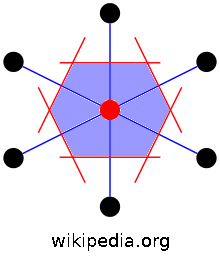
\includegraphics[width=2cm]{glossary/images/wsc.png}}}
}
\newglossaryentry{brillouinzone}
{
    name={Brillouin Zone},
    description={the Wigner-Seitz cell in reciprocal space}
}

\newglossaryentry{wavefunction}
{
    name={wave function},
    description={contains all there is to know about a system and it's meaning is given by a probability ${\lvert \Psi \rvert}^2 = 1 $}
}

\newglossaryentry{planewave}
{
    name={plane wave},
    description={a wave of parallel planes of constant frequency that are normal to the direction of propagation}
}

\newglossaryentry{blochtheorem}
{
    name={Bloch theorem},
    description={electron wave functions may be written as a sum of plane waves $\psi_{\vec{k},n} \vec{r} = \sum c_{\vec{k} + \vec{G}, n} exp(i (\vec{k} + \vec{G}) \dot \vec{r})$}
}

\newglossaryentry{atomicunits}
{
    name={Atomic Units},
    description={length in Bohr - 1 bohr = 0.529 angstrom, energy in Hartree - 1 Hartree = 27.211 eV}
}
\newglossaryentry{jellium}
{
    name={jellium},
    description={quantum mechanical model of electrons distributed uniformly through space (homogeneous electron gas)}
}
\newglossaryentry{heg}
{
    name={homogeneous electron gas},
    description={quantum mechanical model of electrons distributed uniformly through space (jellium)}
}
\newglossaryentry{304SS}
{
    name={304SS},
    description={Austenitic stainless steel: 18-20\%Cr, 8-11\%Ni}
}
\newglossaryentry{316SS}
{
    name={316SS},
    description={Austenitic stainless steel: 16.5-18.5\%Cr, 10-13\%Ni, 2.0-2.5\%Mo}
}
\newglossaryentry{matrixdiagonalization}
{
    name={matrix diagonalization},
    description={Take matrix $A$ and find a diagonal matrix $D$ such that $S^-1 A S = D$}
}
\newglossaryentry{supercritical}
{
    name=supercritical,
    description={Above $374^{\circ}C$ (647K) and 22.1MPa water is no longer a distinct liquid or gas and it becomes supercritical}
}
\newglossaryentry{reduction}
{
    name=reduction,
    description={Gaining electrons or loss of oxygen}
}
\newglossaryentry{oxidation}
{
    name=oxidation,
    description={Losing electrons or gaining oxygen}
}
\newglossaryentry{cathode}
{
    name=cathode,
    description={Electrode where current enters from an electrolyte}
}
\newglossaryentry{anode}
{
    name=anode,
    description={Electrode where current leaves to an electrolyte}
}
\newglossaryentry{valenceelectron}
{
    name=valence electron,
    description={outer shell electron that can form bonds}
}
\newglossaryentry{kohnshameq}
{
    name=Kohn-Sham equations,
    description={$\hat{v}_{KS}(\vec{r_e}, \vec{r_n}) = v_{n-e}(\vec{r_e}, \vec{r_n}) + \int d^3\vec{r'} \frac{\rho(\vec{r_{e}'})}{\lvert \vec{r_{e}} - \vec{r_{e}'}} + v_{xc}[\rho](\vec{r_{e}})$}
}
\newglossaryentry{pauliexp}
{
    name=Pauli exclusion principle,
    description={half-integer spin particles cannot have the same quantum numbers}
}
\newglossaryentry{paulivector}
{
    name=Pauli vector,
    description={sum of the three Pauli matrices $\vec{\sigma} = \begin{bmatrix} 0 & 1 \\ 1 & 0\end{bmatrix} + \begin{bmatrix} 0 & -i \\ i & 0\end{bmatrix} + \begin{bmatrix} 1 & 0 \\ 0 & -1\end{bmatrix}$}
}
\newglossaryentry{fermion}
{
    name=fermion,
    description={half-integer spin particle - includes electrons, protons, neutrons}
}
\newglossaryentry{boson}
{
    name=boson,
    description={integer spin particle - includes photons, gluons}
}
\newglossaryentry{proofstrength}
{
    name=proof strength,
    description={stress at which a material undergoes a permanent extension}
}
\newglossaryentry{youngsmodulus}
{
    name=Young's modulus,
    description={measure of resistance to elastic deformation $\delta = \frac{\text{stress}}{\text{strain}}$}
}
\newglossaryentry{yieldstrength}
{
    name=yield strength,
    description={maximum stress before permanent deformation occurs}
}
\newglossaryentry{ultimatetensilestrength}
{
    name=ultimate tensile strength,
    description={maximum stress the material can withstand}
}
\newglossaryentry{allotrope}
{
    name=allotrope,
    description={an element that exists in multiple forms/structures - the common example of allotropes are graphite (hexagonal sheets) and diamond (regular tetrahedral structure) for carbon}
}
\newglossaryentry{obsstable}
{
    name=observationally stable,
    description={theoretically unstable but yet to be measured as unstable by experiment}
}




%%%%%%%%%%%%%%%%%%%%%%%%%%%%%%%%%%%
% Elements
%%%%%%%%%%%%%%%%%%%%%%%%%%%%%%%%%%%

\newglossaryentry{C}
{
    name=C,
    description={Carbon $Z = 6$, $A_r = 12.00$}
}
\newglossaryentry{Mg}
{
    name=Mg,
    description={Magnesium $Z = 12$, $A_r = 24.30$}
}
\newglossaryentry{P}
{
    name=P,
    description={Phosphorus $Z = 15$, $A_r = 30.97$}
}
\newglossaryentry{Cr}
{
    name=Cr,
    description={Chromium $Z = 24$, $A_r = 52.00$}
}
\newglossaryentry{Mn}
{
    name=Mn,
    description={Maganese $Z = 25$, $A_r = 54.94$}
}
\newglossaryentry{Fe}
{
    name=Fe,
    description={Iron $Z = 26$, $A_r = 55.85$}
}
\newglossaryentry{Co}
{
    name=Co,
    description={Cobalt $Z = 27$, $A_r = 58.93$}
}
\newglossaryentry{Ni}
{
    name=Ni,
    description={Nickel $Z = 28$, $A_r = 58.69$}
}
\newglossaryentry{Cu}
{
    name=Cu,
    description={Copper $Z = 29$, $A_r = 63.55$}
}
\newglossaryentry{Zr}
{
    name=Zr,
    description={Zirconium $Z = 40$, $A_r = 91.22$}
}
\newglossaryentry{Mo}
{
    name=Mo,
    description={Molybdenum $Z = 42$, $A_r = 95.95$}
}
\newglossaryentry{Ru}
{
    name=Ru,
    description={Ruthenium $Z = 44$, $A_r = 101.07$}
}
\newglossaryentry{Pd}
{
    name=Pd,
    description={Palladium $Z = 46$, $A_r = 106.42$}
}
\newglossaryentry{W}
{
    name=W,
    description={Tungsten $Z = 74$, $A_r = 183.84$}
}
\newglossaryentry{Ir}
{
    name=Ir,
    description={Iridium $Z = 77$, $A_r = 192.22$}
}
\newglossaryentry{Pt}
{
    name=Pt,
    description={Platinum $Z = 78$, $A_r = 195.08$}
}
\newglossaryentry{Th}
{
    name=Th,
    description={Thorium $Z = 90$, $A_r = 232.04$}
}
\newglossaryentry{U}
{
    name=U,
    description={Uranium $Z = 92$, $A_r = 238.03$}
}
\newglossaryentry{Pu}
{
    name=Pu,
    description={Plutonium $Z = 94$, $A_r = 244$}
}


%%%%%%%%%%%%%%%%%%%%%%%%%%%%%%%%%%%
% Radiation Units
%%%%%%%%%%%%%%%%%%%%%%%%%%%%%%%%%%%

\newglossaryentry{becquerel}
{
    name=Becquerel,
    description={Becquerel (Bq) - decays per second}
}
\newglossaryentry{curie}
{
    name=Curie,
    description={Curie (Ci) - activity of 1 gram of Radium-226 - 1Ci = $3.7 \times 10^{10}$ decays per second}
}
\newglossaryentry{rutherford}
{
    name=Rutherford,
    description={Rutherford (Rd) - $1.0 \times 10^{6}$ decays per second}
}
\newglossaryentry{rontgen}
{
    name=Rontgen,
    description={Rontgen (R) - a measure of electric charge freed per unit mass of air - $1R = 2.58 \times 10^{-4} C/kg$}
}
\newglossaryentry{gray}
{
    name=Gray,
    description={Gray (Gy) how much energy is deposited into matter and 1Gy is equal to 1 Joule per kg}
}
\newglossaryentry{rad}
{
    name=Rad,
    description={Rad (Rad) this is another measure for absorbed dose and 1 rad is equal to 100 ergs per gram (1 rad = 1.0cGy = 0.01Gy)}
}
\newglossaryentry{sievert}
{
    name=Sievert,
    description={Sievert (Sv) - equivalent/effective dose - this is the absorbed dose with radiation weighting (equivalent) and tissue weighting (effective) factors applied $1Sv \text{(equivalent)} = 1 J/kg \times W_r$ and $1Sv \text{(effective)} = 1 J/kg \times W_r \times W_t$}
}
\newglossaryentry{rem}
{
    name=Rontgen Equivalent Man,
    description={Rontgen Equivalent Man (REM) - equivalent/effective dose - 1 REM equivalent is equal to $1Rad \times W_r$ (1cGy $1Rad \times W_r$) and 1 REM effective is equal to $1Rad \times W_r \times W_t$ (1cGy $1Rad \times W_r \times W_t$)}
}
\newglossaryentry{ld50}
{
    name=LD50,
    description={Lethal dose in 50 percent of cases}
}
\newglossaryentry{barn}
{
    name=barn,
    description={Unit for cross sectional area ($1.0 \times 10^{28} m^{2}$)}
}
\newglossaryentry{meanfreepath}
{
    name=mean free path,
    description={average (mean) distance a projectile travels before reacting with the target}
}



\newacronym{kerma}{KERMA}{Kinetic Energy Released per unit MAss}

\newacronym{gif}{GIF}{Generation IV International Forum}
\newacronym{geniv}{GenIV}{Generation IV}


\newacronym{gen1}{Gen I}{Generation I}
\newacronym{gen2}{Gen II}{Generation II}
\newacronym{gen2+}{Gen II+}{Generation II+}
\newacronym{gen3}{Gen III}{Generation III}
\newacronym{gen3+}{Gen III+}{Generation III+}
\newacronym{gen4}{Gen IV}{Generation IV}

\newacronym{pwr}{PWR}{Pressurised Water Reactor}
\newacronym{lwr}{LWR}{Light Water Reactor}
\newacronym{bwr}{BWR}{Boiling Water Reactor}
\newacronym{agr}{AGR}{Advanced Gas Reactor}
\newacronym{vver}{VVER}{Vodo-Vodyanoi Energetichesky Reaktor}
\newacronym{rbmk}{RBMK}{Reaktor Bolshoy Moshchnosti Kanalnyy}
\newacronym{candu}{CANDU}{Canada Deuterium Uranium}
\newacronym{epr}{EPR}{European Pressurised Reactor}
\newacronym{abwr}{ABWR}{Advanced Boiling Water Reactor}
\newacronym{gfr}{GFR}{Gas-Cooled Fast Reactor}
\newacronym{lfr}{LFR}{Lead-Cooled Fast Reactor}
\newacronym{msr}{MSR}{Molten Salt Reactor}
\newacronym{scwr}{SCWR}{Supercritical-Water-Cooled Reactor}
\newacronym{sfr}{SFR}{Sodium-Cooled Fast Reactor}
\newacronym{vhtr}{VHTR}{Very-High-Temperature Reactor}
\newacronym{fnr}{FNR}{Fast-Neutron Reactors}
\newacronym{elsy}{ELSY}{European Lead Fast Reactor}
\newacronym{fbr}{FBR}{Fast Breeder Reactor}
\newacronym{pbr}{PBR}{Pebble-Bed Reactor}
\newacronym{npp}{NPP}{Nuclear Power Plant}
\newacronym{ebr}{EBR}{Experimental Breeder Reactor}
\newacronym{iter}{ITER}{International Thermonuclear Experimental Reactor}
\newacronym{hpr}{HPR}{Hualong Pressurised Water Reactor}

\newacronym{ecis}{ECIS}{Equations Couplées Itérations Séquentielle}


\newacronym{triso}{TRISO}{Tristructural Isotropic}

\newacronym{ccgt}{CCGT}{Combined Cycle Gas Turbine}


\newacronym{endf}{ENDF}{Evaluated Nuclear Data File}
\newacronym{nea}{NEA}{Nuclear Energy Agency}
\newacronym{jeff}{JEFF}{Joint Evaluated Fission and Fusion File}
\newacronym{tendl}{TENDL}{TALYS-based Evaluated Nuclear Data Library}


\newacronym{sc}{SC}{Simple Cubic}
\newacronym{bcc}{BCC}{body centered cubic}
\newacronym{fcc}{FCC}{face centered cubic}
\newacronym{fct}{FCT}{face centered tetragonal}
\newacronym{cph}{CPH}{face centered tetragonal}
\newacronym{hcp}{HCP}{hexagonal close packed}
\newacronym{zb}{ZB}{zinc blende}


\newacronym{mcnp}{MCNP}{Monte Carlo N-Particle}

\newacronym{hrb}{HRB}{Hardness Rockwell B}


\newacronym{md}{MD}{molecular dynamics}
\newacronym{akmc}{akMC}{atomic kinetic Monte Carlo}
\newacronym{lammps}{LAMMPS}{Large-scale Atomic/Molecular Massively Parallel Simulator}


\newacronym{nist}{NIST}{National Institute of Standards and Technology}

\newacronym{fs}{FS}{Finnis-Sinclair}
\newacronym{eam}{EAM}{embedded-atom method}
\newacronym{2beam}{2BEAM}{two band embedded-atom method}
\newacronym{meam}{MEAM}{modified embedded-atom method}

\newacronym{hf}{HF}{Hartree-Fock}

\newacronym{dft}{DFT}{Density Functional Theory}
\newacronym{scf}{SCF}{self consistent field}
\newacronym{pbe}{PBE}{Perdew-Burke-Ernzerhof}
\newacronym{pbesol}{PBESOL}{Perdew-Burke-Ernzerhof functional revised for solids}
\newacronym{pz}{PZ}{Perdew-Zunger}
\newacronym{lda}{LDA}{local density approximation}
\newacronym{lsda}{LSDA}{local spin density approximation}
\newacronym{gga}{GGA}{generalized gradient approximation}
\newacronym{zbl}{ZBL}{Ziegler-Biersack-Littmark}

\newacronym{igscc}{IGSCC}{inter granular stress corrosion cracking}
\newacronym{tgscc}{TGSCC}{trans granular stress corrosion cracking}
\newacronym{iascc}{IASCC}{irradiation assisted stress corrosion cracking}
\newacronym{scc}{SCC}{stress corrosion cracking}
\newacronym{ris}{RIS}{radiation induced segregation}
\newacronym{rip}{RIP}{radiation induced precipitation}

\newacronym{dpa}{DPA}{displacements per atom}
\newacronym{vpi}{VPI}{vacancies per ion}
\newacronym{pka}{PKA}{primary knock-on atom}


\newacronym{edf}{EDF}{Électricité de France}


\newacronym{cpu}{CPU}{central processing unit}
\newacronym{gpu}{GPU}{graphical processing unit}

\newacronym{pgm}{PGM}{platinum group metal}


\newacronym{ornl}{ORNL}{Oak Ridge National Laboratory}
\newacronym{linac}{LINAC}{linear accelerator}
\newacronym{sns}{SNS}{Spallation Neutron Source}
\newacronym{rfq}{RFQ}{Radio Frequency Quadrupole}
\newacronym{hfir}{HFIR}{High Flux Isotope Reactor}
\newacronym{slac}{SLAC}{Stanford Linear Accelerator Center}
\newacronym{triumf}{TRIUMF}{TRI-University Meson Facility}
\newacronym{lhc}{LHC}{Large Hadron Collider}
\newacronym{cern}{CERN}{Conseil Européen pour la Recherche Nucléaire}
\newacronym{nbs}{NBS}{National Bureau of Standards}
\newacronym{nbsr}{NBSR}{National Bureau of Standards Reactor}
\newacronym{avf}{AVF}{Azimuthally Varying Field}
\newacronym{iaea}{IAEA}{International Atomic Energy Agency}


\newacronym{ins}{INS}{Institute for Nuclear Study}



\newacronym{mox}{MOX}{mixed oxide}

\newacronym{srim}{SRIM}{Stopping Range In Matter}
\newacronym{exyz}{EXYZ}{Energy, x, y, z}
\newacronym{trim}{TRIM}{TRansport In Matter}
\newacronym{nds}{NDS}{Nuclear Data Services}

\newacronym{omp}{OMP}{optical model potential}
\newacronym{nomp}{NOMP}{nuclear optical model potential}


\newacronym{exfor}{EXFOR}{EXchange FORmat}


\newacronym{bca}{BCA}{binary collision approximation}



\newacronym{tise}{TISE}{Time Independent Schr\"{o}dinger Equation}
\newacronym{hk}{HK}{Hohenberg-Kohn}
\newacronym{ks}{KS}{Kohn-Sham}
\newacronym{xc}{XC}{exchange-correlation}


\newacronym{ng}{NG}{Newton-Gauss}
\newacronym{lma}{LMA}{Levenberg-Marquardt Algorithm}
\newacronym{bfgs}{BFGS}{Broyden Fletcher Goldfarb Shanno}
\newacronym{lmbfgs}{LM-BFGS}{Limited-memory Broyden Fletcher Goldfarb Shanno}
\newacronym{nm}{NM}{Nelder Mead}
\newacronym{sa}{SA}{Simulated Annealing}
\newacronym{bh}{BH}{Basin Hopping}
\newacronym{cg}{CG}{Conjugate Gradient}
\newacronym{qp}{QP}{Quadratric Programming}





\newacronym{ecp}{ECP}{electrochemical corrosion potential}

\newacronym{eos}{EOS}{equation of state}
\newacronym{ec}{EC}{elastic constants}
\newacronym{mskp}{MSKP}{Mehl, Singh, Klein, Papaconstantopoulos}
\newacronym{rfkj}{RFKJ}{Ravindran, Fast, Korzhavyi, Johansson}

\newacronym{dna}{DNA}{Deoxyribonucleic Acid}


\newacronym{ke}{KE}{Kirkendall effect}
\newacronym{ike}{IKE}{inverse Kirkendall effect}

\newacronym{asme}{ASME}{American Society of Engineers}

\newacronym{sem}{SEM}{scanning electron microscope}
\newacronym{tem}{TEM}{transmission electron microscope}
\newacronym{stem}{STEM}{scanning transmission electron microscope}
\newacronym{sims}{SIMS}{secondary-ion mass spectrometry}
\newacronym{naa}{NAA}{neutron activation analysis}

\newacronym{bz}{BZ}{Brillouin zone}
\newacronym{ibz}{IBZ}{irreducible Brillouin zone}


\newacronym{rss}{RSS}{residual squared sum}

\newacronym{url}{URL}{Uniform Resource Locator}
\newacronym{www}{WWW}{World Wide Web}

\newacronym{uk}{UK}{United Kingdom}
\newacronym{usa}{USA}{United States of America}
\newacronym{ussr}{USSR}{United Socialist Soviet Republic}


\makeglossaries